%\documentclass[12pt]{article}
%\usepackage[a4paper, margin=1in]{geometry} 
%\usepackage{graphicx} 
%\usepackage{hyperref}
%\usepackage{float}
%\usepackage[font=small, labelfont=bf]{caption}

%\begin{document}

%
% Introduction to Biotechnology
%
\subsection{Introduction to Biotechnology}
Biotechnology is the use of laboratory techniques to study living organism and cells. 

%
% Applications of biotechnology
%
\subsubsection*{Applications of biotechnology}
Branches of biotechnology can be explained with different colors.
\begin{itemize}
\item Red: medical processes
\item Green: agricultural processes
\item White: industrial processes
\item Blue: marine and aquatic applications
\end{itemize}

%
% Laboratory tools and equipment
%
\subsubsection*{Laboratory tools and equipment}

\begin{figure}[H]
  \centering
      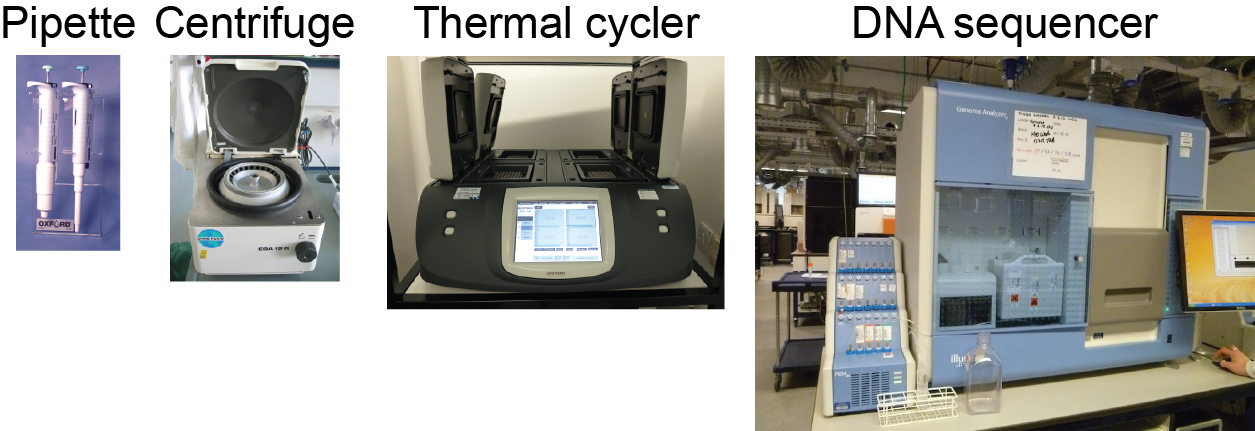
\includegraphics[width=0.5\textwidth]{fig01/lab_equipment.png}
  \caption{Pipette, centrifuge, thermal cycler, and DNA sequencer \newline (sources:  \href{https://en.wikipedia.org/wiki/Pipette\#/media/File:Single_channel_rack.jpg}{Domain}, \href{https://commons.wikimedia.org/w/index.php?curid=494}{Manske},
\href{https://commons.wikimedia.org/w/index.php?curid=20189025}{Rror}, 
\href{https://commons.wikimedia.org/w/index.php?curid=18862968}{RE73} via Wikimedia Commons)}
\end{figure}
 
%
% Human genome project
%
\subsubsection*{Human genome project}
It was a large-scale international research project to determine the whole DNA sequences of human.

\begin{itemize}
\item 1990 –- 2003
\item \$2.7 billion
\end{itemize}

%
% Next generation sequencing
%
\subsubsection*{Next generation sequencing}
Sequence technologies have been rapidly advanced since the human genome project.

Example: sequence a whole human genome with Illumina HiSeq X Ten.
\begin{itemize}
\item One day
\item \$1000
\end{itemize}

%
% Protein sequencing
%
\subsubsection*{Protein sequencing}
Proteins are generally more studied than DNAs and RNAs, but the whole proteome is generally harder to analyze than the whole genome. MS (mass-spectrometry) based technologies are widely used to sequence proteins.

\begin{figure}[H]
  \centering
      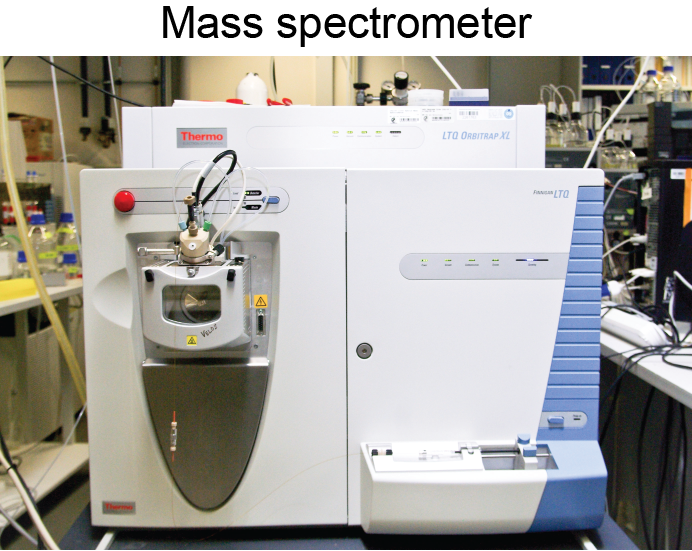
\includegraphics[width=0.25\textwidth]{fig01/mass_spectrometer.png}
  \caption{Orbitrap mass spectrometer (source: \href{https://commons.wikimedia.org/w/index.php?curid=18691799}{Wi\`{o}rkiewicz, Wikimedia Commons})}
\end{figure}
 
%\end{document}
